\documentclass[conference]{IEEEtran}
\IEEEoverridecommandlockouts
% The preceding line is only needed to identify funding in the first footnote. If that is unneeded, please comment it out.
\usepackage{cite}
\usepackage{amsmath,amssymb,amsfonts}
\usepackage{algorithmic}
\usepackage{graphicx}
\usepackage{textcomp}
\usepackage{xcolor}
\usepackage[utf8]{inputenc}
\usepackage[english]{babel}
\usepackage{hyperref}

\urlstyle{same}
\def\BibTeX{{\rm B\kern-.05em{\sc i\kern-.025em b}\kern-.08em
    T\kern-.1667em\lower.7ex\hbox{E}\kern-.125emX}}
\begin{document}

\title{Fall Detection System Using \\Sensors Embedded In Smartphones}



\author{\IEEEauthorblockN{ Vineeth Bhat}
\IEEEauthorblockA{\textit{Dept.Computer Science and Engineering} \\
\textit{Frankfurt University of Applied Sciences}\\
Frankfurt, Germany \\
vineeth.bhat@stud.fra-uas.de}
\and
\IEEEauthorblockN{Jathin Sreenivas}
\IEEEauthorblockA{\textit{Dept.Computer Science and Engineering} \\
\textit{Frankfurt University of Applied Sciences}\\
Frankfurt, Germany \\
Jathin.Sreenivas@stud.fra-uas.de}
\and
\IEEEauthorblockN{Vidya Gopalakrishnarao}
\IEEEauthorblockA{\textit{Dept.Computer Science and Engineering} \\
\textit{Frankfurt University of Applied Sciences}\\
Frankfurt, Germany \\
vidya.gopalakrishnarao@stud.fra-uas.de}
}




\maketitle

\begin{abstract}
This document is an introduction to the project Human Activity Recognition(HAR). The scope of the project is to understand the working of the sensors in our smartphones or tablet and access it to track various human activity like walking, jogging, etc and propose a system(application) that detects fall.
\end{abstract}

\section{Project Vision}
Our smartphones are filled with sensors that read various data from the physical world around them. These data is then utilised by various application on the smartphone as per their need. The objective of this project is to provide an application that detects fall, when a person falls while he is walking or jogging.\\
We are building an application that access the sensors embedded in our smartphones that are necessary to monitor the human activity and collect the data acquired by the sensor, there by utilising it to detect the fall. \\
The idea behind this project is to monitor the sensors like accelerometer, gyroscope for abnormal or irregular readings while running or walking which follows a particular pattern, when this reading is recorded the system will start a counter for specified time to check if there is any further activity for example back to walking, from the person who has fallen down, if there is no activity from that person then within that predefined time-frame the system will trigger an alert that is a message to a chosen contact as emergency contact, that this person is in danger and in need of help. For the second case if there is an activity for example, just the device has fallen and the person has picked up the device or he has fallen but he is not hurt able to walk back home safely and resumes the normal activity within that predefined time then the system will not trigger an alert message to the emergency contact. 

\section{Requirements}
\subsection{Functional Requirements}
\begin{itemize}
\item Accessing the sensor using the system's operating system to obtain the data.
\item Determine the fall based on the readings from the sensors and use the predefined time to detect any further activity and decide the future action.
\item Create an alarm on the device if fall has occurred.
\item Message service to the emergency contact provided based on the fall recognition from the user's smartphone.
\item Sending the current location of the user along with distress signal.
\item Authentication from the user that he is fine, in the form of an alert message asking him if he is fine. If there is no response from the user then it is considered that he is in distress and alert will be triggered.
\item Visualisation of data. That is representing the data collected in readable form.
\end{itemize}

\subsection{Non- Functional Requirements}
\begin{itemize}
\item Primary requirement is to detect fall in a person, using appropriate sensors embedded in the smart phone.
\item Real time monitoring of human activity.
\item Accurate measurement of the activity by the sensor..
\item Appropriate alert message to the emergency contact.
\item Accurate tracking of location.
\item The application must adapt varying display sizes of mobile screen.
\item User friendly UI/UX.\\
\end{itemize}

\begin{figure}
\centerline{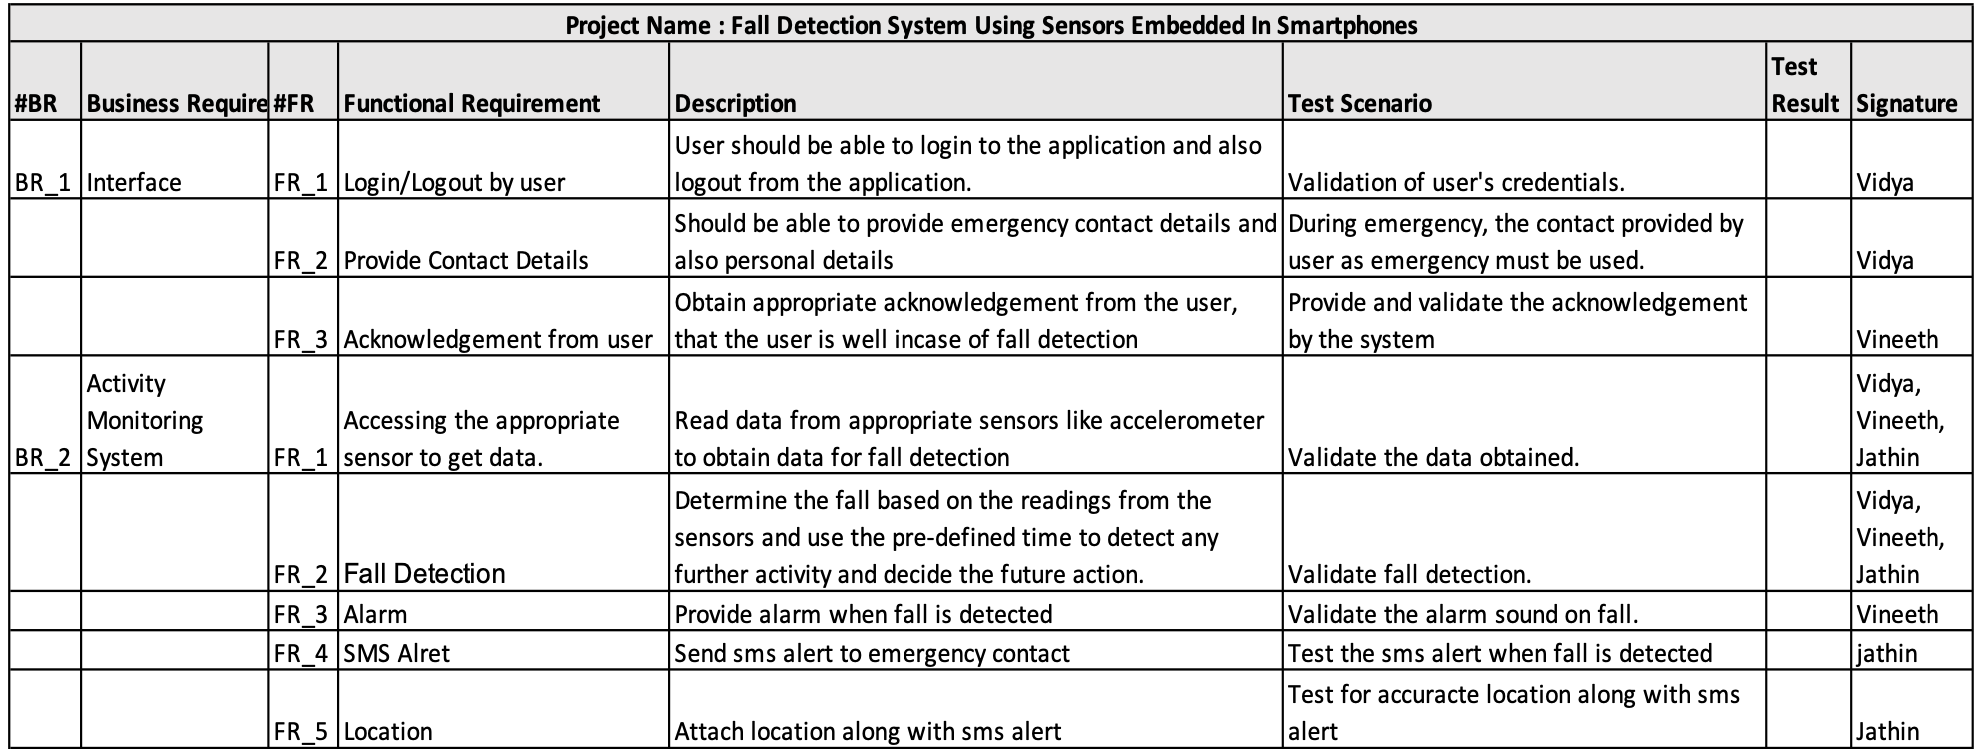
\includegraphics[width=9cm,height=4cm]{RTM.png}}
\caption{Requirement Tracebility Matrix}
\label{fig2}
\end{figure}

\section{Project Estimation}

 We are using Function Point Analysis and COCOMO model to predict the development time and effort for our project.The actual time required to develop this project will be based on the source lines of code, which is calculated by  counting the number of inputs, outputs, inquiries, master files, interfaces required and also the Unadjusted Function Points. Finally, we will get 1609.3 lines of code from the calculation, considering the language factor for JAVA which is assumed to be 38. The development time will be 4.2156 months/person or 3.955 person/month.\cite{b4}
 \begin{itemize}
\item Source Lines of Code: SLOC = 1609.3
\item Programmer Productivity:PM = 3.95530 person/month
\item Development time: DEV = 4.2156 months
\end{itemize}

\section{Responsibilities of all team members}
Figure.~\ref{fig3} shows the responsibility of all team members.The whole team is involved in major activities such as requirement analysis, design and Implementation.The activities such as project vision, cost estimation and testing is handled individually.  
\begin{figure}
\centerline{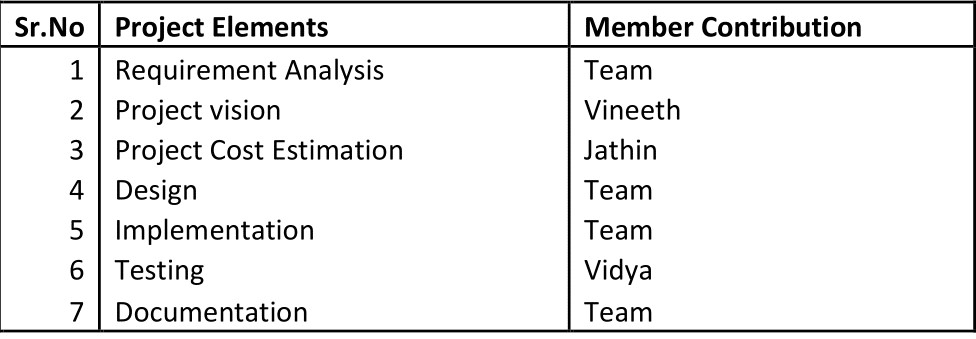
\includegraphics[width=9cm,height=4cm]{resourceUtilization.png}}
\caption{Resource Utilization}
\label{fig3}
\end{figure}

\section{Security}
\begin{itemize}
\item Privacy of user information. Example location, login data.
\item Confidentiality of the data collected from the sensor.
\item Requesting access permission to monitor the activity and device features.
\item User authentication for accessing the app and data. 
\item Sensor data can not be accessed from outside the Smartphone.
\end{itemize}

\section{Reliability}
\begin{itemize}
\item Accurate detection of fall based on sensor readings.
\item The data collected from the sensor must be reliable for any further use.
\item Activity monitored must be accurate.
\item Capability to handle large amount of data and perform as intended.
\item State of the application is uninterrupted by external interruption.
\end{itemize}

\section{Project Design}
Considering the above mentioned requirements we have hashed out following design for our projects.

\subsection{Use Case Diagram}
Figure.~\ref{usecase} shows the interaction of application with the user. Since the application detects fall based on sensor reading and activity tracking, we have kept the user interaction to a minimal. User logins to the application and provides the emergency details. Apart from this the main feature would be checking the well being of the user in case of fall detected, in the form of an acknowledgement from user.

\subsection{Sequence Diagram}
To understand the object interaction in a time sequence, we designed the following sequence diagram (Figure.~\ref{sequenceDiagram}) for our project. User, UI, Activity Monitoring System and Emergency contact are involved in the interaction. User initiates the Activity Monitoring System by logging into the application and providing emergency contact details. Once initiated the system tracks the activity and detects fall, in case of any the system requests the user for an acknowledgement that he is able to carry on. Here there are two possible cases. Case 1: If user confirms that he is well and that it is a false alarm then the system will not trigger alert to emergency contact. Case 2: If the user does not acknowledge, then the system considers the user has fallen down and needs assistant and contacts the emergency contact.

\begin{figure}
\centerline{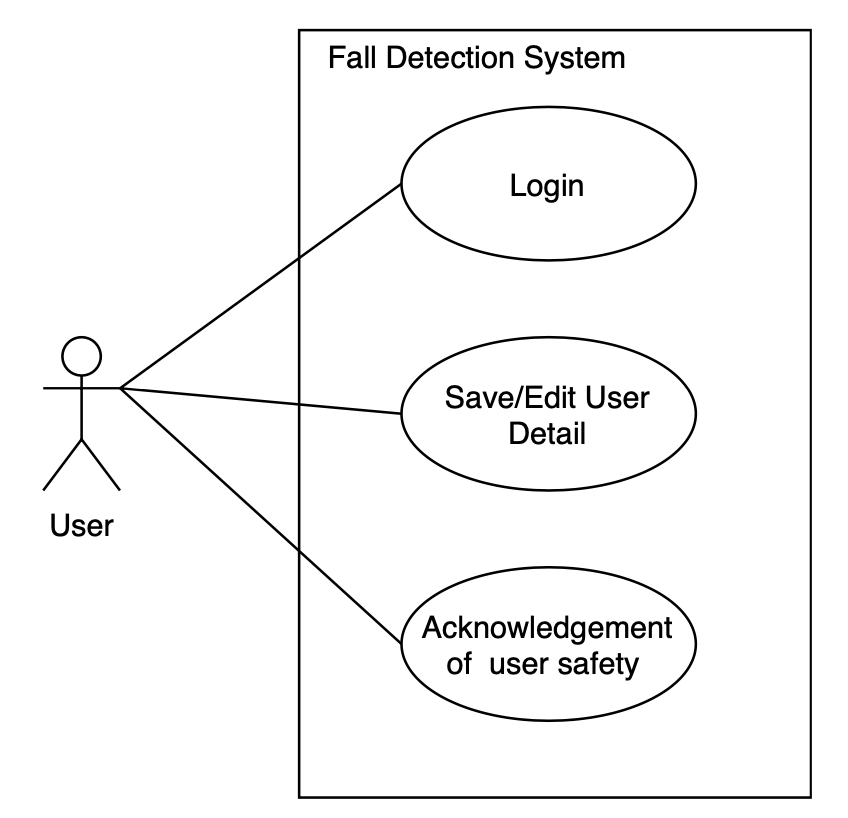
\includegraphics[width=6cm, height=6cm]{usecase.png}}
\caption{Use case diagram}
\label{usecase}
\end{figure}

\begin{figure}
\centerline{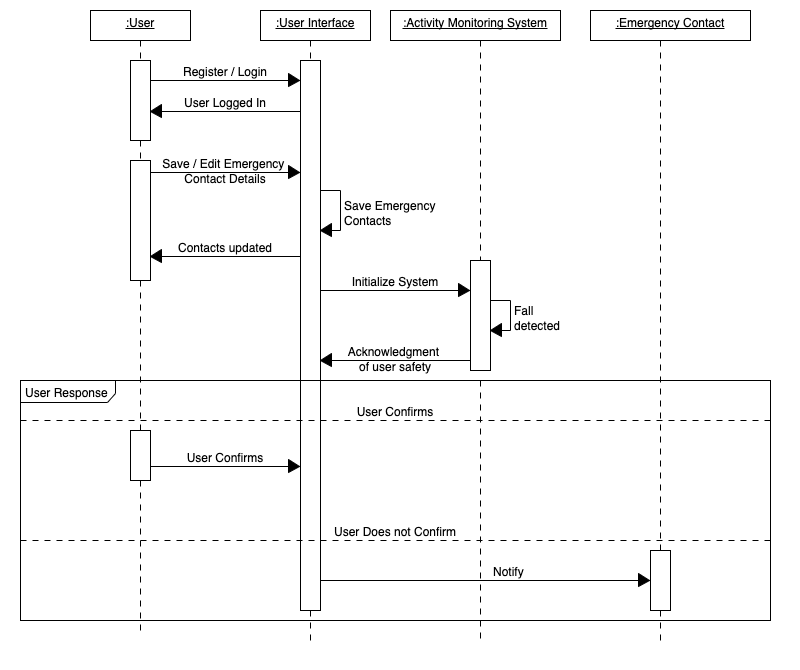
\includegraphics[width=8cm, height=7cm]{sequenceDiagram.png}}
\caption{Sequence Diagram}
\label{sequenceDiagram}
\end{figure} 

\subsection{Class Diagram}
Figure.~\ref{classDiagram} explains the project architecture, explaining the class files and the functions involved in the project.

\begin{figure}
\centerline{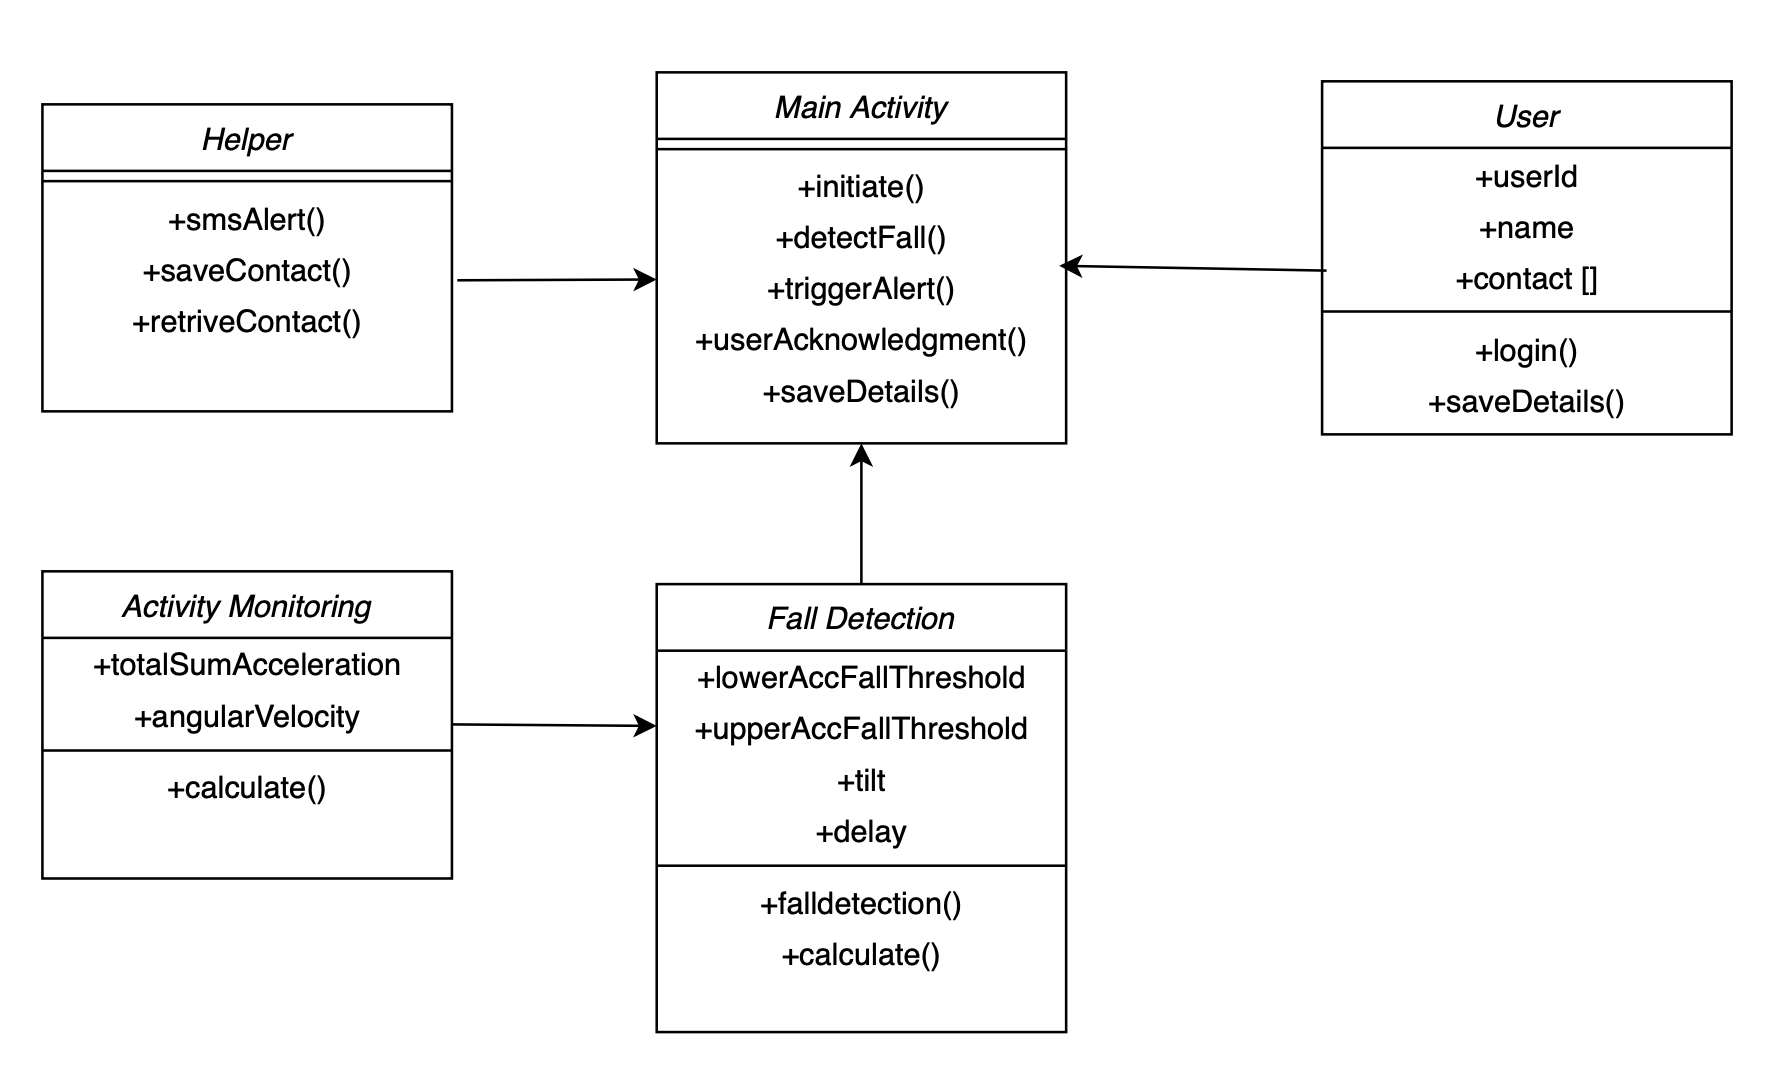
\includegraphics[width=8cm, height=6cm]{classDiagram.png}}
\caption{Class Diagram}
\label{classDiagram}
\end{figure}

\section{Development Environment}
As we are using android devices in our team, for this we are considering the android as our development environment.\\
Using Android sensor framework we can access the available sensors and acquire the raw sensor data. Android provides dedicated hardware package for accessing the embedded sensors. It includes the following classes and interface, SensorManager, Sensor, SensorEvent, SensorEventListner.

\subsection{Sensor Framework}
The sensor framework provides certain classes and interface to perform variety of sensor related tasks. For example, finding out the available sensors on the device.\\

The package that includes sensor framework is android.hardware. It provides following classes and interface to access the sensors,
\begin{itemize}
    \item SensorManager: This class is used to create an instance of the sensor service. It provides methods for accessing, listening and perform various action on the sensors.
    \item Sensor: This class is used to create an instance of a specific sensor.Sensor's capabilities are determined by this class.
    \item SensorEvent: Using this class the system creates a sensor event object, which is used to get information about the sensors. It include the following information, raw sensor data, type of the sensor that generated the event, timestamp, accuracy.
    \item SensorEventListener: Using this interface we can create two callback methods that receive notification when sensor values change or when sensor accuracy changes.
\end{itemize}
In a basic application we use these classes and interface to perform following tasks, identifying sensor and sensor capabilities and monitor sensor events.\\

\section{Hardware and Software}
Following list specifies the hardware and software used in our project.
\begin{itemize}
    \item Smartphone: Google Pixel
    \item Operating System: Android
    \item IDE: Android Studio
    \item Version Control: GitHub
\end{itemize}
\subsection{Sensor}
There are 3 categories of sensors,
\begin{itemize}
    \item Motion Sensors: These sensors are responsible for monitoring the acceleration force and rotational forces along the three axes. This category includes,gravity sensors, accelerometers, gyroscopes and rotational vector sensors.
    \item Position Sensors: Physical positioning of the device is measured b these sensors. These sensors include orientation sensors and magnetometer. 
    \item Environmental Sensors: Environmental parameters such as temperature, pressure, illumination and humidity are measured using these sensors. This includes, barometer, photometer and thermometer.
\end{itemize}

\subsection{Sensors Used}
There are various number of sensors that the android platform provides, for our project we'll be using the following sensors,\\
Accelerometer: Acceleration is the measurement of the rate of change in velocity, the accelerometer is an electromechanical device that is used for measuring acceleration forces. In the case of a sensor present in a mobile device, dynamic to sense movement or vibration. The accelerometer can operate in two ways the piezoelectric effect and the capacitance sensor. The Piezoelectric accelerometer uses microscopic crystal structures that become "squeezed" due to forces. These crystals create a voltage when squeezed and accelerometer interprets this voltage to determine the acceleration. Whereas the capacitance accelerometer changes the capacitance between microstructures located next to the device. If an accelerative force moves any of these structures the capacitance changes and accelerometer will read the capacitance and translates to a voltage for interpretation. In the android device the accelerometer measures the acceleration that is applied to a device on all three axes (x, y, and z), including the force of gravity. We are using this sensor to track the movement of the phone, and also to track the orientation and acceleration force of the device. In our application the acceleration along all the 3 axes in m2/s and the corresponding graph will be displayed, so if the phone is moved in any direction, the data and graph will change accordingly in real-time.\\
Gyroscope: The gyroscope sensor is a device that can measure and maintain the orientation and angular velocity of an object. They are more advanced than accelerometers. Accelerometers can measure only linear motion, whereas a gyroscope can measure tilt and lateral orientation. The Coriolis force concept is used in the Gyroscope sensors. To measure the angular rate, the rotation rate of the sensor is converted into an electrical signal. Measures a device's rate of rotation around each of the three physical axes (x, y, and z). A gyroscope can be used for navigation and measurement of angular velocity. In our application we will show the orientation along the three 3 axes in rad/s along with the corresponding graph.

\section{Fall Detection Algorithm}
The application uses a threshold based algorithm to detect falls. Threshold based algorithms are preferred as these algorithms require low computational cost and lower complexity. This fall detection algorithm as depicted in (Figure.~\ref{fig:fallDetectAlgo}), defines several parameters depending on the accelerometer and gyroscope outputs, and a decision is made using the threshold values for these parameters. The parameters used in the algorithm are The total sum acceleration vector \(SV\) and The angular velocity \(\theta\). The total sum acceleration vector is calculated by
\begin{equation}
 SV = \sqrt{(A_x)^2 + (A_y)^2 + (A_z)^2}\label{eq:1}
 \end{equation}
 
where \(A_x\), \(A_y\) and \(A_z\) are the reading from the accelerometer along the x,y and z axes. The angular velocity \(\theta\) is calculated by 
\begin{equation}
\theta = \sqrt{(\omega_x)^2 + (\omega_y)^2 + (\omega_z)^2}\label{eq:2}
\end{equation}

where \(\omega_x\), \(\omega_y\) and \(\omega_z\) are readings from the gyroscope along the x, y and z axes.

When the user falls, the \(SV\) calculated using (Equation.~\ref{eq:1}) changes rapidly and the \(\theta\) calculated using (Equation.~\ref{eq:2}) also increases along the fall direction. This application uses 4 thresholds vales to determine a fall.
\begin{itemize}
    \item FT1 (lower acceleration threshold): When the user starts to fall down, the acceleration starts decreasing. There is a significant change in \(SV\). 
    \item FT2 (time-delay):  When the user falls down, the application checks if user is down for FT2 seconds, to avoid false detection like if the user is bending down or if user wakes up after fall. 
    \item FT3 (upper acceleration threshold): This corresponds to value after user hits the floor, which is a large pike on how hard the user has fallen down to the ground. FT3 is set to value more than 1.8g which is the impact of the user on the ground. 
    \item FT4 (tilt): Corresponds to the tilt when the user falls on the floor. FT4 is set to a value greater than 70deg which proves that user has actually is down on the ground and avoids false detection such as if user sits on the sofa. If the calculated \(\theta\) exceeds FT4 then it can be a a possible fall.
\end{itemize}

At the end if the application has detected a fall and but the user was not effected because of the fall, to avoid a alarm in these cases the application brings up a notification for the user to acknowledge to confirm if the user has not fallen. If the user acknowledges that he has not fallen, the emergency contact is not notified, else a SMS sent to the emergency contact which comprises of the address of the user's location. 
 
\begin{figure}
\centerline{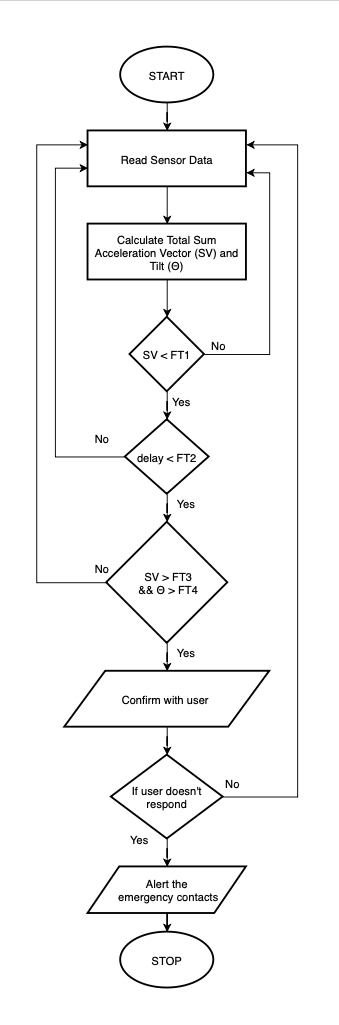
\includegraphics[width=5cm, height=11cm]{Flowchart.png}}
\caption{Fall Detection Algorithm Flowchart}
\label{fig:fallDetectAlgo}
\end{figure}

\begin{thebibliography}{00}
\bibitem{b1} Sensors: https://developer.android.com/guide/topics/sensors Accessed: 09.06.2020
\bibitem{b2} Gyroscope:
https://ef.engr.utk.edu/hyperphysics/hbase/gyr.html Accessed: 09.06.2020
\bibitem{b3} Live Science: https://www.livescience.com/40102-accelerometers.html Accessed: 09.06.2020
\bibitem{b4} Cost Estimation, Padmaja,  http://people.cs.ksu.edu/~padmaja/Project/CostEstimate.html,  Accessed: 09.06.2020
\bibitem{b5}E. Thammasat and J. Chaicharn, "A simply fall-detection algorithm using accelerometers on a smartphone," The 5th 2012 Biomedical Engineering International Conference, Ubon Ratchathani, 2012, pp. 1-4, doi: 10.1109/BMEiCon.2012.6465471.
\bibitem{b6}F. Sposaro and G. Tyson, "iFall: An android application for fall monitoring and response," 2009 Annual International Conference of the IEEE Engineering in Medicine and Biology Society, Minneapolis, MN, 2009, pp. 6119-6122, doi: 10.1109/IEMBS.2009.5334912.
\bibitem{b7}S. Abdelhedi, R. Bourguiba, J. Mouine and M. Baklouti, "Development of a two-threshold-based fall detection algorithm for elderly health monitoring," 2016 IEEE Tenth International Conference on Research Challenges in Information Science (RCIS), Grenoble, 2016, pp. 1-5, doi: 10.1109/RCIS.2016.7549315.
\bibitem{b8}Bourke, Alan \& ÓLaighin, Gearóid. (2008). A threshold-based fall-detection algorithm using a bi-axial gyroscope sensor. Medical engineering \& physics. 30. 84-90. 10.1016/j.medengphy.2006.12.001.
\bibitem{b9}H. W. Guo, Y. T. Hsieh, Y. S. Huang, J. C. Chien, K. Haraikawa and J. S. Shieh, "A threshold-based algorithm of fall detection using a wearable device with tri-axial accelerometer and gyroscope," 2015 International Conference on Intelligent Informatics and Biomedical Sciences (ICIIBMS), Okinawa, 2015, pp. 54-57, doi: 10.1109/ICIIBMS.2015.7439470.

\end{thebibliography}
\vspace{12pt}

\end{document}
